\documentclass[ignorenonframetext,]{beamer}
\setbeamertemplate{caption}[numbered]
\setbeamertemplate{caption label separator}{: }
\setbeamercolor{caption name}{fg=normal text.fg}
\beamertemplatenavigationsymbolsempty
\usepackage{lmodern}
\usepackage{amssymb,amsmath}
\usepackage{ifxetex,ifluatex}
\usepackage{fixltx2e} % provides \textsubscript
\ifnum 0\ifxetex 1\fi\ifluatex 1\fi=0 % if pdftex
\usepackage[T1]{fontenc}
\usepackage[utf8]{inputenc}
\else % if luatex or xelatex
\ifxetex
\usepackage{mathspec}
\else
\usepackage{fontspec}
\fi
\defaultfontfeatures{Ligatures=TeX,Scale=MatchLowercase}
\fi
\usetheme{metropolis}
% use upquote if available, for straight quotes in verbatim environments
\IfFileExists{upquote.sty}{\usepackage{upquote}}{}
% use microtype if available
\IfFileExists{microtype.sty}{%
\usepackage{microtype}
\UseMicrotypeSet[protrusion]{basicmath} % disable protrusion for tt fonts
}{}
\newif\ifbibliography
\usepackage{color}
\usepackage{fancyvrb}
\newcommand{\VerbBar}{|}
\newcommand{\VERB}{\Verb[commandchars=\\\{\}]}
\DefineVerbatimEnvironment{Highlighting}{Verbatim}{commandchars=\\\{\}}
% Add ',fontsize=\small' for more characters per line
\usepackage{framed}
\definecolor{shadecolor}{RGB}{248,248,248}
\newenvironment{Shaded}{\begin{snugshade}}{\end{snugshade}}
\newcommand{\KeywordTok}[1]{\textcolor[rgb]{0.13,0.29,0.53}{\textbf{{#1}}}}
\newcommand{\DataTypeTok}[1]{\textcolor[rgb]{0.13,0.29,0.53}{{#1}}}
\newcommand{\DecValTok}[1]{\textcolor[rgb]{0.00,0.00,0.81}{{#1}}}
\newcommand{\BaseNTok}[1]{\textcolor[rgb]{0.00,0.00,0.81}{{#1}}}
\newcommand{\FloatTok}[1]{\textcolor[rgb]{0.00,0.00,0.81}{{#1}}}
\newcommand{\ConstantTok}[1]{\textcolor[rgb]{0.00,0.00,0.00}{{#1}}}
\newcommand{\CharTok}[1]{\textcolor[rgb]{0.31,0.60,0.02}{{#1}}}
\newcommand{\SpecialCharTok}[1]{\textcolor[rgb]{0.00,0.00,0.00}{{#1}}}
\newcommand{\StringTok}[1]{\textcolor[rgb]{0.31,0.60,0.02}{{#1}}}
\newcommand{\VerbatimStringTok}[1]{\textcolor[rgb]{0.31,0.60,0.02}{{#1}}}
\newcommand{\SpecialStringTok}[1]{\textcolor[rgb]{0.31,0.60,0.02}{{#1}}}
\newcommand{\ImportTok}[1]{{#1}}
\newcommand{\CommentTok}[1]{\textcolor[rgb]{0.56,0.35,0.01}{\textit{{#1}}}}
\newcommand{\DocumentationTok}[1]{\textcolor[rgb]{0.56,0.35,0.01}{\textbf{\textit{{#1}}}}}
\newcommand{\AnnotationTok}[1]{\textcolor[rgb]{0.56,0.35,0.01}{\textbf{\textit{{#1}}}}}
\newcommand{\CommentVarTok}[1]{\textcolor[rgb]{0.56,0.35,0.01}{\textbf{\textit{{#1}}}}}
\newcommand{\OtherTok}[1]{\textcolor[rgb]{0.56,0.35,0.01}{{#1}}}
\newcommand{\FunctionTok}[1]{\textcolor[rgb]{0.00,0.00,0.00}{{#1}}}
\newcommand{\VariableTok}[1]{\textcolor[rgb]{0.00,0.00,0.00}{{#1}}}
\newcommand{\ControlFlowTok}[1]{\textcolor[rgb]{0.13,0.29,0.53}{\textbf{{#1}}}}
\newcommand{\OperatorTok}[1]{\textcolor[rgb]{0.81,0.36,0.00}{\textbf{{#1}}}}
\newcommand{\BuiltInTok}[1]{{#1}}
\newcommand{\ExtensionTok}[1]{{#1}}
\newcommand{\PreprocessorTok}[1]{\textcolor[rgb]{0.56,0.35,0.01}{\textit{{#1}}}}
\newcommand{\AttributeTok}[1]{\textcolor[rgb]{0.77,0.63,0.00}{{#1}}}
\newcommand{\RegionMarkerTok}[1]{{#1}}
\newcommand{\InformationTok}[1]{\textcolor[rgb]{0.56,0.35,0.01}{\textbf{\textit{{#1}}}}}
\newcommand{\WarningTok}[1]{\textcolor[rgb]{0.56,0.35,0.01}{\textbf{\textit{{#1}}}}}
\newcommand{\AlertTok}[1]{\textcolor[rgb]{0.94,0.16,0.16}{{#1}}}
\newcommand{\ErrorTok}[1]{\textcolor[rgb]{0.64,0.00,0.00}{\textbf{{#1}}}}
\newcommand{\NormalTok}[1]{{#1}}

% Prevent slide breaks in the middle of a paragraph:
\widowpenalties 1 10000
\raggedbottom

\AtBeginPart{
\let\insertpartnumber\relax
\let\partname\relax
\frame{\partpage}
}
\AtBeginSection{
\ifbibliography
\else
\let\insertsectionnumber\relax
\let\sectionname\relax
\frame{\sectionpage}
\fi
}
\AtBeginSubsection{
\let\insertsubsectionnumber\relax
\let\subsectionname\relax
\frame{\subsectionpage}
}

\setlength{\parindent}{0pt}
\setlength{\parskip}{6pt plus 2pt minus 1pt}
\setlength{\emergencystretch}{3em}  % prevent overfull lines
\providecommand{\tightlist}{%
\setlength{\itemsep}{0pt}\setlength{\parskip}{0pt}}
\setcounter{secnumdepth}{0}

\title{Chapter 1: The Basics}
\author{Tyson S. Barrett}
\date{Summer 2017}

\begin{document}
\frame{\titlepage}

\begin{frame}
\tableofcontents[hideallsubsections]
\end{frame}

\section{Introduction}\label{introduction}

\begin{frame}

\centerline{
\includegraphics[height=1.5in]{Figures/Rlogo.png} \text{  \LARGE and    }

\includegraphics[height=1.5in]{Figures/RStudio_logo.png}}

\vspace{6pt}

\centering
This class will use R and RStudio to show how R can make several aspects
of your research simpler, more likely to be reproducible, and more
replicable.

\end{frame}

\begin{frame}{Data Types, Objects and More}

In this chapter we will discuss:

\begin{itemize}[<+->]
\tightlist
\item
  data types and objects,
\item
  importing data, and
\item
  saving data.
\end{itemize}

\emph{These aspects of R, although maybe mundane, are important for: 1)
Data manipulation, 2) Modeling, and 3) Output.}

\end{frame}

\section{Objects}\label{objects}

\begin{frame}{Physical Objects}

\textbf{For Example:}

\vspace{6pt}\centerline{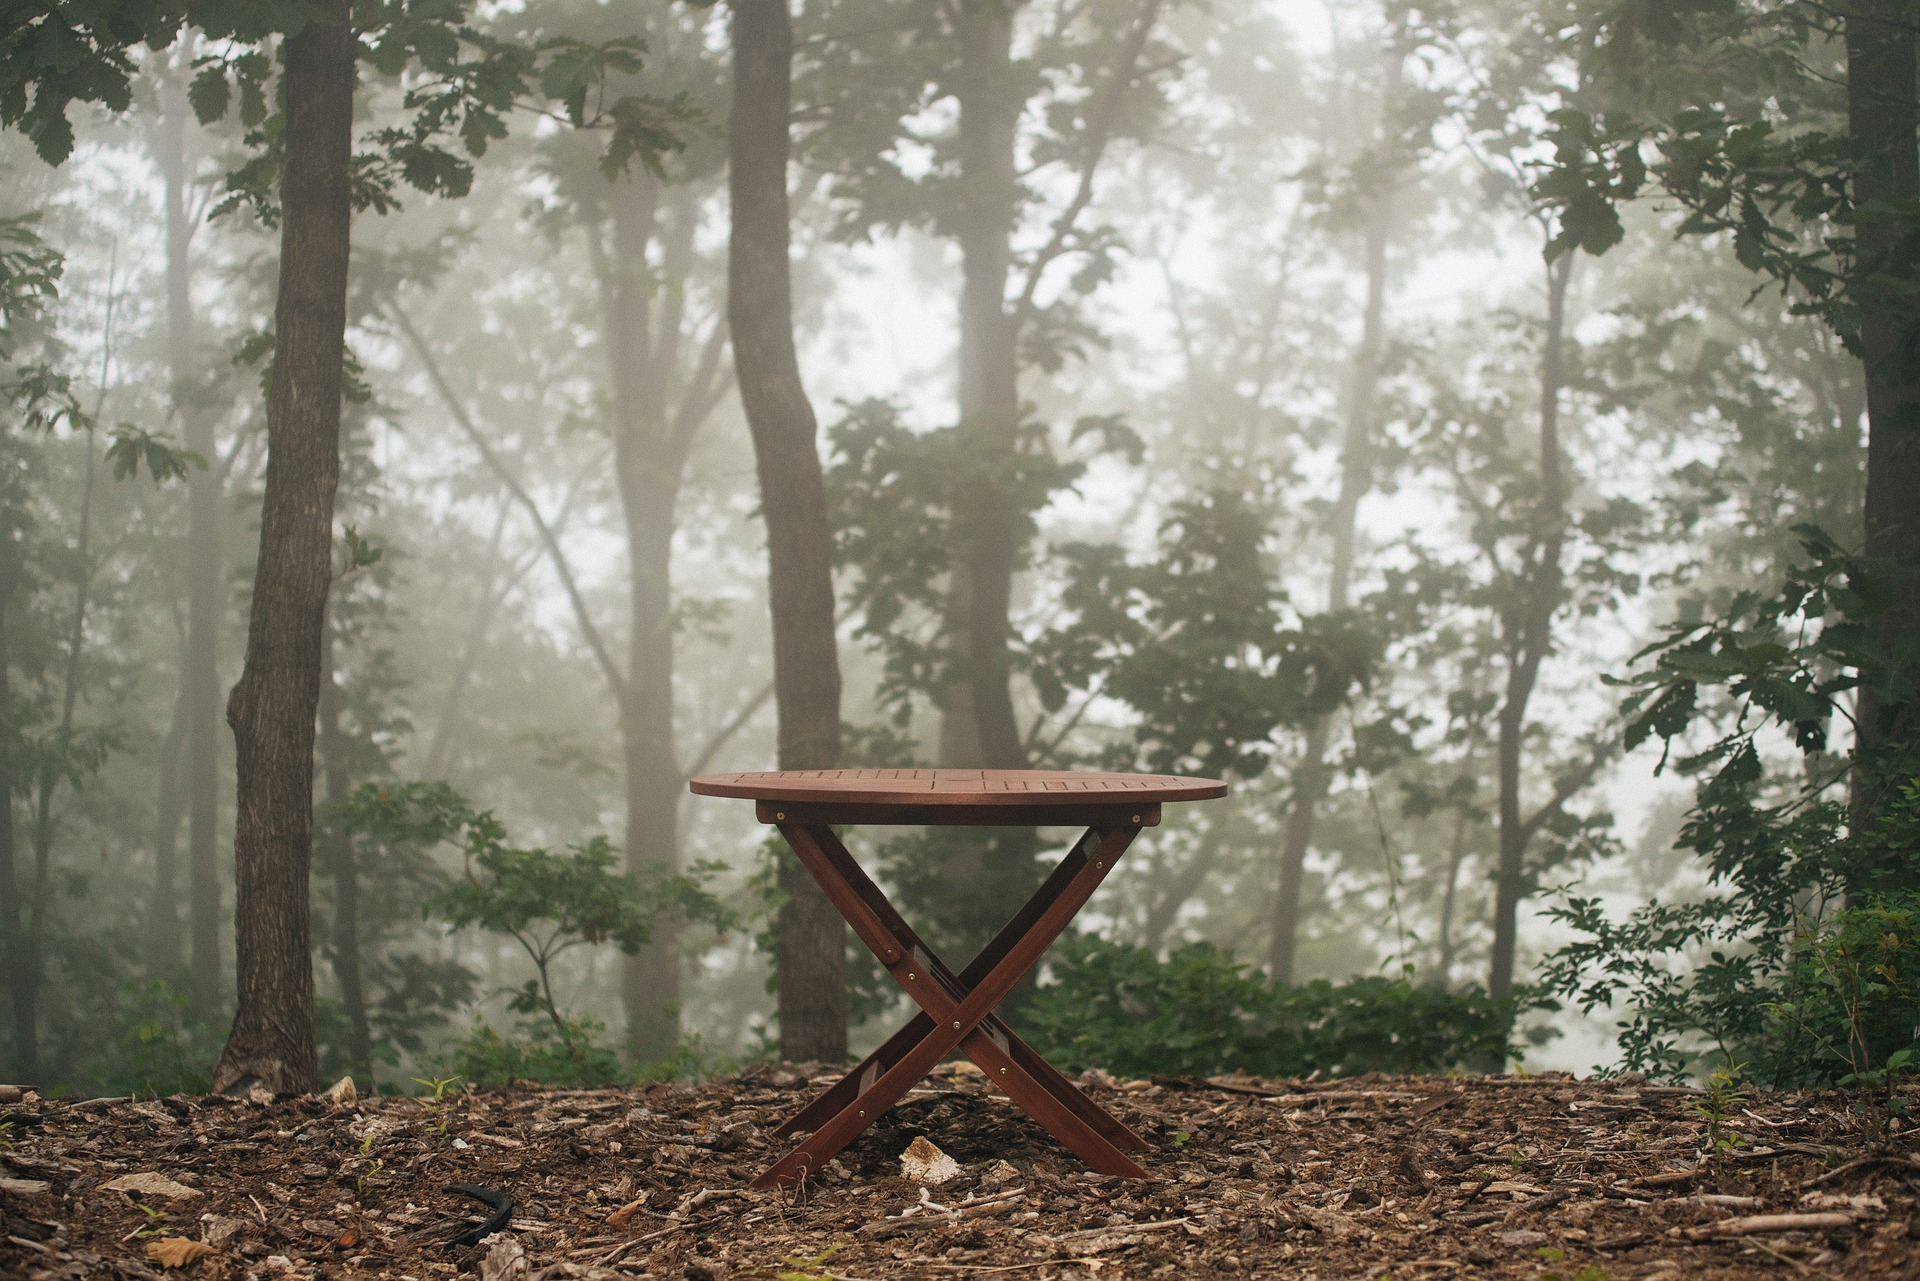
\includegraphics[height=2in]{Figures/table_forest.jpg}}

\begin{itemize}
\tightlist
\item
  A table is great to eat on, write on, and somewhat good at sitting on.
\item
  But it is horrible at taking you from Los Angeles to Toronto.
\end{itemize}

\end{frame}

\begin{frame}[fragile]{Virtual Objects}

Likewise, objects in \texttt{R} are useful for some things and not for
others. Objects are how we interact with the data, analyze it, and
output it.

We will discuss the most important objects for working with data:

\begin{itemize}[<+->]
\tightlist
\item
  Vectors
\item
  Data Frames
\item
  Lists
\end{itemize}

\end{frame}

\section{Data Types: Vectors}\label{data-types-vectors}

\begin{frame}[fragile]{\texttt{numeric}}

\texttt{numeric} is a vector with numbers.\footnote<.->{the \texttt{c()}
  is a function that glues the numbers (or whatever else is in the
  parenthases) together} It can be whole numbers (i.e.~an
\texttt{integer}) or any real number (i.e. \texttt{double}). Below is a
\texttt{double}.

\begin{Shaded}
\begin{Highlighting}[]
\NormalTok{x <-}\StringTok{ }\KeywordTok{c}\NormalTok{(}\FloatTok{10.1}\NormalTok{, }\FloatTok{2.1}\NormalTok{, }\FloatTok{4.6}\NormalTok{, }\FloatTok{2.3}\NormalTok{, }\FloatTok{8.9}\NormalTok{)}
\NormalTok{x}
\end{Highlighting}
\end{Shaded}

\begin{verbatim}
[1] 10.1  2.1  4.6  2.3  8.9
\end{verbatim}

Here, x, is the so-called ``pointer'' of this vector. So by typing the
name of the object, we can see the contents.

\end{frame}

\begin{frame}[fragile]{\texttt{character}}

A \texttt{character} vector is essentially just letters or words.

\begin{Shaded}
\begin{Highlighting}[]
\NormalTok{ch <-}\StringTok{ }\KeywordTok{c}\NormalTok{(}\StringTok{"I think this is great."}\NormalTok{, }
        \StringTok{"I would suggest you learn R."}\NormalTok{, }
        \StringTok{"You seem quite smart."}\NormalTok{)}
\NormalTok{ch}
\end{Highlighting}
\end{Shaded}

\begin{verbatim}
[1] "I think this is great."       "I would suggest you learn R."
[3] "You seem quite smart."       
\end{verbatim}

\end{frame}

\begin{frame}[fragile]{\texttt{factor}}

A \texttt{factor} is a special vector in \texttt{R} for categorical
variables. It is actually stored as numbers but we can give it
labels.\footnote<.->{Note that before we used the \texttt{factor()}
  function, the race object was just \texttt{numeric}. Once we told it
  was a ``factor'' \texttt{R} treats it as categorical.}

\begin{Shaded}
\begin{Highlighting}[]
\NormalTok{race <-}\StringTok{ }\KeywordTok{c}\NormalTok{(}\DecValTok{1}\NormalTok{, }\DecValTok{3}\NormalTok{, }\DecValTok{2}\NormalTok{, }\DecValTok{1}\NormalTok{, }\DecValTok{1}\NormalTok{, }\DecValTok{2}\NormalTok{, }\DecValTok{1}\NormalTok{, }\DecValTok{3}\NormalTok{, }\DecValTok{4}\NormalTok{, }\DecValTok{2}\NormalTok{)}
\NormalTok{race <-}\StringTok{ }\KeywordTok{factor}\NormalTok{(race, }
               \DataTypeTok{labels =} \KeywordTok{c}\NormalTok{(}\StringTok{"white"}\NormalTok{, }\StringTok{"black"}\NormalTok{, }
                          \StringTok{"hispanic"}\NormalTok{, }\StringTok{"asian"}\NormalTok{))}
\NormalTok{race}
\end{Highlighting}
\end{Shaded}

\begin{verbatim}
 [1] white    hispanic black    white    white    black    white   
 [8] hispanic asian    black   
Levels: white black hispanic asian
\end{verbatim}

\end{frame}

\section{Data Types: Data Frames and
Lists}\label{data-types-data-frames-and-lists}

\begin{frame}[fragile]{Data Frames}

The \texttt{data.frame} is the most important data type for most
projects.\footnote<.->{We can do quite a bit with the
  \texttt{data.frame} that we called \texttt{df}. (Once again, we could
  have called it anything, although I recommend short names.)}

\begin{Shaded}
\begin{Highlighting}[]
\NormalTok{df <-}\StringTok{ }\KeywordTok{data.frame}\NormalTok{(}\StringTok{"A"} \NormalTok{=}\StringTok{ }\KeywordTok{c}\NormalTok{(}\DecValTok{1}\NormalTok{,}\DecValTok{2}\NormalTok{,}\DecValTok{1}\NormalTok{,}\DecValTok{4}\NormalTok{,}\DecValTok{3}\NormalTok{),}
                 \StringTok{"B"} \NormalTok{=}\StringTok{ }\KeywordTok{c}\NormalTok{(}\FloatTok{1.4}\NormalTok{,}\FloatTok{2.1}\NormalTok{,}\FloatTok{4.6}\NormalTok{,}\FloatTok{2.0}\NormalTok{,}\FloatTok{8.2}\NormalTok{),}
                 \StringTok{"C"} \NormalTok{=}\StringTok{ }\KeywordTok{c}\NormalTok{(}\DecValTok{0}\NormalTok{,}\DecValTok{0}\NormalTok{,}\DecValTok{1}\NormalTok{,}\DecValTok{1}\NormalTok{,}\DecValTok{1}\NormalTok{))}
\NormalTok{df}
\end{Highlighting}
\end{Shaded}

\begin{verbatim}
  A   B C
1 1 1.4 0
2 2 2.1 0
3 1 4.6 1
4 4 2.0 1
5 3 8.2 1
\end{verbatim}

\end{frame}

\begin{frame}[fragile]{Data Frames}

If ``A'' and ``C'' are factors we can tell \texttt{R} by:

\begin{Shaded}
\begin{Highlighting}[]
\NormalTok{df$A <-}\StringTok{ }\KeywordTok{factor}\NormalTok{(df$A, }\DataTypeTok{labels =} \KeywordTok{c}\NormalTok{(}\StringTok{"level1"}\NormalTok{, }\StringTok{"level2"}\NormalTok{, }
                                \StringTok{"level3"}\NormalTok{, }\StringTok{"level4"}\NormalTok{))}
\NormalTok{df$C <-}\StringTok{ }\KeywordTok{factor}\NormalTok{(df$C, }\DataTypeTok{labels =} \KeywordTok{c}\NormalTok{(}\StringTok{"Male"}\NormalTok{, }\StringTok{"Female"}\NormalTok{))}
\end{Highlighting}
\end{Shaded}

In the above code, the \texttt{\$} reaches into \texttt{df} to grab a
variable (i.e.~column).

\end{frame}

\begin{frame}[fragile]{Data Frames}

The following code does the exact same thing:\footnote<.->{There are
  actually very small differences but its really not important here.}

\begin{Shaded}
\begin{Highlighting}[]
\NormalTok{df[[}\StringTok{"A"}\NormalTok{]] <-}\StringTok{ }\KeywordTok{factor}\NormalTok{(df$A, }\DataTypeTok{labels =} \KeywordTok{c}\NormalTok{(}\StringTok{"level1"}\NormalTok{, }\StringTok{"level2"}\NormalTok{, }
                                     \StringTok{"level3"}\NormalTok{, }\StringTok{"level4"}\NormalTok{))}
\NormalTok{df[[}\StringTok{"C"}\NormalTok{]] <-}\StringTok{ }\KeywordTok{factor}\NormalTok{(df$C, }\DataTypeTok{labels =} \KeywordTok{c}\NormalTok{(}\StringTok{"Male"}\NormalTok{, }\StringTok{"Female"}\NormalTok{))}
\end{Highlighting}
\end{Shaded}

and so is the following:

\begin{Shaded}
\begin{Highlighting}[]
\NormalTok{df[, }\StringTok{"A"}\NormalTok{] <-}\StringTok{ }\KeywordTok{factor}\NormalTok{(df$A, }\DataTypeTok{labels =} \KeywordTok{c}\NormalTok{(}\StringTok{"level1"}\NormalTok{, }\StringTok{"level2"}\NormalTok{, }
                                     \StringTok{"level3"}\NormalTok{, }\StringTok{"level4"}\NormalTok{))}
\NormalTok{df[, }\StringTok{"C"}\NormalTok{] <-}\StringTok{ }\KeywordTok{factor}\NormalTok{(df$C, }\DataTypeTok{labels =} \KeywordTok{c}\NormalTok{(}\StringTok{"Male"}\NormalTok{, }\StringTok{"Female"}\NormalTok{))}
\end{Highlighting}
\end{Shaded}

\end{frame}

\begin{frame}[fragile]{Data Frames}

On the previous slide:

\begin{itemize}[<+->]
\tightlist
\item
  \texttt{df{[}{[}"A"{]}{]}} grabs the \texttt{A} variable just like
  \texttt{df\$A}. The last example shows that we can grab both columns
  and rows.
\item
  In \texttt{df{[},\ "C"{]}} we have a spot just a head of the comma. It
  works like this: \texttt{df{[}rows,\ columns{]}}.
\end{itemize}

\begin{Shaded}
\begin{Highlighting}[]
\NormalTok{df[}\DecValTok{1}\NormalTok{:}\DecValTok{3}\NormalTok{, }\StringTok{"A"}\NormalTok{]}
\NormalTok{df[}\DecValTok{1}\NormalTok{:}\DecValTok{3}\NormalTok{, }\DecValTok{1}\NormalTok{]}
\end{Highlighting}
\end{Shaded}

\begin{itemize}[<+->]
\tightlist
\item
  Both lines of the above code grabs rows 1 thorugh 3 and column ``A''.
\end{itemize}

\end{frame}

\begin{frame}[fragile]{Data Frames}

Finally, we can combine the \texttt{c()} function to grab different rows
and columns. To grab rows 1 and 5 and columns ``B'' and ``C'' you can do
the following:

\begin{Shaded}
\begin{Highlighting}[]
\NormalTok{df[}\KeywordTok{c}\NormalTok{(}\DecValTok{1}\NormalTok{,}\DecValTok{5}\NormalTok{), }\KeywordTok{c}\NormalTok{(}\StringTok{"B"}\NormalTok{, }\StringTok{"C"}\NormalTok{)]}
\end{Highlighting}
\end{Shaded}

\end{frame}

\begin{frame}[fragile]{Some Functions for Data Frames}

\emph{Get the names of the variables:}

\begin{Shaded}
\begin{Highlighting}[]
\KeywordTok{names}\NormalTok{(df)}
\end{Highlighting}
\end{Shaded}

\begin{verbatim}
[1] "A" "B" "C"
\end{verbatim}

\emph{Know what type of variable it is:}

\begin{Shaded}
\begin{Highlighting}[]
\KeywordTok{class}\NormalTok{(df$A)}
\end{Highlighting}
\end{Shaded}

\begin{verbatim}
[1] "factor"
\end{verbatim}

\end{frame}

\begin{frame}[fragile]{Some Functions for Data Frames}

\emph{Get quick summary statistics for each variable:}

\begin{Shaded}
\begin{Highlighting}[]
\KeywordTok{summary}\NormalTok{(df)}
\end{Highlighting}
\end{Shaded}

\begin{verbatim}
      A           B             C    
 level1:2   Min.   :1.40   Male  :2  
 level2:1   1st Qu.:2.00   Female:3  
 level3:1   Median :2.10             
 level4:1   Mean   :3.66             
            3rd Qu.:4.60             
            Max.   :8.20             
\end{verbatim}

\end{frame}

\begin{frame}[fragile]{Some Functions for Data Frames}

*Get the first 10 columns of your \url{data:*}

\begin{Shaded}
\begin{Highlighting}[]
\KeywordTok{head}\NormalTok{(df, }\DataTypeTok{n=}\DecValTok{10}\NormalTok{)}
\end{Highlighting}
\end{Shaded}

\begin{verbatim}
       A   B      C
1 level1 1.4   Male
2 level2 2.1   Male
3 level1 4.6 Female
4 level4 2.0 Female
5 level3 8.2 Female
\end{verbatim}

\end{frame}

\section{Importing Data}\label{importing-data}

\begin{frame}[fragile]{Import, Don't Input}

Most of the time you'll want to import data into \texttt{R} rather than
manually entering it line by line, variable by variable.

There are some built in ways to import many delimited\footnote<.->{The
  delimiter is what separates the pieces of data.} data types
(e.g.~comma delimited--also called a CSV, tab delimited, space
delimited). Other \textbf{packages}\footnote<.->{A package is an
  extension to \texttt{R} that gives you more functions--abilities--to
  work with data. Anyone can write a package, although to get it on the
  Comprehensive R Archive Network (CRAN) it needs to be vetted to a
  large degree. In fact, after some practice, you could write a package
  to help you more easily do your work.} have been developed to help
with this as well.

\end{frame}

\begin{frame}{Important Note about Importing}

When you import data into R, it does not do anything to the data file
(unless you ask it to). So, you can play around with it in R, change its
shape, subset it, and whatever else you'd like without destroying or
even modifying the original data.

Note that the slides that discuss \textbf{saving data} show you how you
can override (not recommended) or save additional data files.

\end{frame}

\begin{frame}[fragile]{Importing Data}

The first, if it is an \texttt{R} data file in the form \texttt{.rda} or
\texttt{.RData} simply use:

\begin{Shaded}
\begin{Highlighting}[]
\KeywordTok{load}\NormalTok{(}\StringTok{"file.rda"}\NormalTok{)}
\end{Highlighting}
\end{Shaded}

Note that you don't assign this to a name such as \texttt{df}. Instead,
it loads whatever \texttt{R} objects were saved to it.

\end{frame}

\begin{frame}[fragile]{Delimited Files}

Most delimited files are saved as \texttt{.csv}, \texttt{.txt}, or
\texttt{.dat}. As long as you know the delimiter, this process is easy.

\begin{Shaded}
\begin{Highlighting}[]
\NormalTok{## for csv}
\NormalTok{df <-}\StringTok{ }\KeywordTok{read.table}\NormalTok{(}\StringTok{"file.csv"}\NormalTok{, }\DataTypeTok{sep =} \StringTok{","}\NormalTok{, }\DataTypeTok{header=}\OtherTok{TRUE}\NormalTok{)}
\NormalTok{## for tab delimited}
\NormalTok{df <-}\StringTok{ }\KeywordTok{read.table}\NormalTok{(}\StringTok{"file.txt"}\NormalTok{, }\DataTypeTok{sep =} \StringTok{"}\CharTok{\textbackslash{}t}\StringTok{"}\NormalTok{, }\DataTypeTok{header=}\OtherTok{TRUE}\NormalTok{)}
\NormalTok{## for space delimited}
\NormalTok{df <-}\StringTok{ }\KeywordTok{read.table}\NormalTok{(}\StringTok{"file.txt"}\NormalTok{, }\DataTypeTok{sep =} \StringTok{" "}\NormalTok{, }\DataTypeTok{header=}\OtherTok{TRUE}\NormalTok{)}
\end{Highlighting}
\end{Shaded}

The argument \texttt{sep} tells the function what kind of delimiter the
data has and \texttt{header} tells \texttt{R} if the first row contains
the variable names.

\small
Note that at the end of the lines you see that I left a \textbf{comment}
using \texttt{\#}. Anything after a \texttt{\#} is not read by the
computer; it's just for us humans.

\end{frame}

\begin{frame}[fragile]{Other Data Formats}

Data from other statistical software such as SAS, SPSS, or Stata are
also easy to get into \texttt{R}. We will use two powerful packages:

\begin{enumerate}
\def\labelenumi{\arabic{enumi}.}
\tightlist
\item
  \texttt{haven}
\item
  \texttt{foreign}
\end{enumerate}

To install, simply run:

\begin{Shaded}
\begin{Highlighting}[]
\KeywordTok{install.packages}\NormalTok{(}\StringTok{"packagename"}\NormalTok{)}
\end{Highlighting}
\end{Shaded}

This only needs to be run once on a computer. Then, to use it in a
single \texttt{R} session (i.e.~from when you open \texttt{R} to when
you close it) run:

\begin{Shaded}
\begin{Highlighting}[]
\KeywordTok{library}\NormalTok{(packagename)}
\end{Highlighting}
\end{Shaded}

\end{frame}

\begin{frame}[fragile]{Other Data Formats}

Using these packages, I will show you simple ways to bring your data in
from other formats.

\begin{Shaded}
\begin{Highlighting}[]
\KeywordTok{library}\NormalTok{(haven)}
\NormalTok{## for Stata data}
\NormalTok{df <-}\StringTok{ }\KeywordTok{read_dta}\NormalTok{(}\StringTok{"file.dta"}\NormalTok{)}
\NormalTok{## for SPSS data}
\NormalTok{df <-}\StringTok{ }\KeywordTok{read_spss}\NormalTok{(}\StringTok{"file.sav"}\NormalTok{)}
\NormalTok{## for this type of SAS file}
\NormalTok{df <-}\StringTok{ }\KeywordTok{read_sas}\NormalTok{(}\StringTok{"file.sas7bdat"}\NormalTok{)}
\end{Highlighting}
\end{Shaded}

\begin{Shaded}
\begin{Highlighting}[]
\KeywordTok{library}\NormalTok{(foreign)}
\NormalTok{## for export SAS files}
\NormalTok{df <-}\StringTok{ }\KeywordTok{read.xport}\NormalTok{(}\StringTok{"file.xpt"}\NormalTok{)}
\end{Highlighting}
\end{Shaded}

\end{frame}

\begin{frame}{Data and Questions}

If you have another type of data file to import, online helps found on
sites like www.stackoverflow.com and www.r-bloggers.com often have the
solution.

\end{frame}

\section{Saving Data}\label{saving-data}

\begin{frame}[fragile]{Saving Data}

Finally, there are many ways to save data. Most of the \texttt{read...}
functions have a corresponding \texttt{write...} function.

\begin{Shaded}
\begin{Highlighting}[]
\NormalTok{## to create a CSV data file}
\KeywordTok{write.table}\NormalTok{(df, }\DataTypeTok{file=}\StringTok{"file.csv"}\NormalTok{, }\DataTypeTok{sep =} \StringTok{","}\NormalTok{)}
\end{Highlighting}
\end{Shaded}

\end{frame}

\begin{frame}[fragile]{Saving Data}

\texttt{R} automatically saves missing data as \texttt{NA} since that is
what it is in \texttt{R}. But often when we write a CSV file, we might
want it as blank or some other value. If that's the case, we can add
another argument \texttt{na\ =\ "\ "} after the sep argument.

\end{frame}

\begin{frame}[fragile]{Help Menu in R}

If you ever have questions about the specific arguments that a certain
function has, you can simply run:

\begin{Shaded}
\begin{Highlighting}[]
\NormalTok{?functionname}
\end{Highlighting}
\end{Shaded}

So, if you were curious about the different arguments in
\texttt{write.table} simply run: \texttt{?write.table}. In the pane with
the files, plots, packages, etc. a document will show up to give you
more informaton.

\end{frame}

\section{Conclusions}\label{conclusions}

\begin{frame}[fragile]{R is built for you}

\begin{itemize}
\tightlist
\item
  \texttt{R} is designed to be flexible and do just about anything with
  data that you'll need to do as a researcher.
\item
  With this chapter under your belt, you can now read basic \texttt{R}
  code, import and save your data.
\item
  The next chapter will introduce the ``tidyverse'' of methods that can
  help you join, reshape, summarize, group, and much more.
\end{itemize}

\end{frame}

\begin{frame}

\centerline{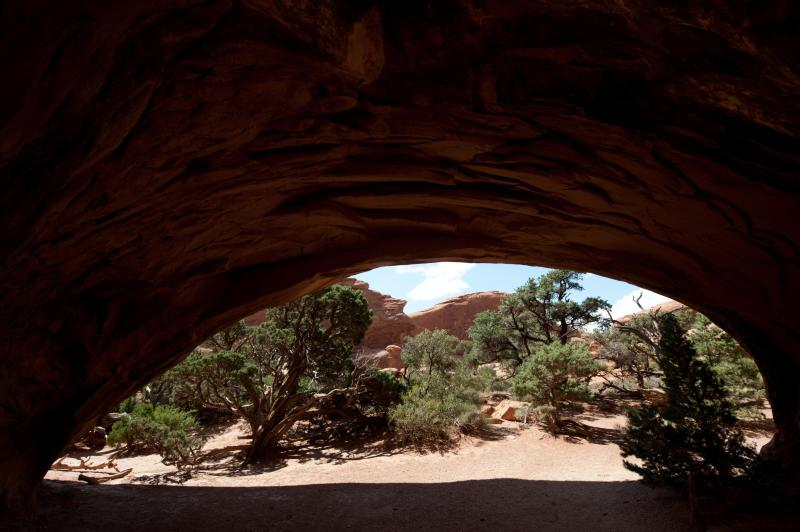
\includegraphics[height=3.9in]{Figures/Navajo_arch.jpg}}

\end{frame}

\end{document}
